
\section{Introduction}\label{sec:1}
\hspace{0.5cm}
Un nouveau cadre pour les calculs neutroniques de base développé à EDF R\&D, dans
le département de SINETICS (SImulation NEutronique, Technologie de l'Information,
Calcul Scientifique) est basé sur la résolution de l'équation de Boltzmann
(ou une approximation) pour les neutrons.\\
Cette équation nécessite en entrée des sections efficaces qui modélisent les
interactions entre les neutrons induits par la fission et les noyaux provenant
soit du combustible soit du modérateur. \\

Ces sections efficaces (au nombre de plusieurs milliers) dépendent
de $d$ paramètres locaux (dits paramètres de rétroaction), tels que la densité de l'eau,
la concentration en bore, la température du carburant, le brûlage du combustible, etc.
Elles sont stockées dans des «bibliothèque nucléaire» et doivent être consultées
régulièrement tout au long de la simulation quand les paramètres de rétroaction évoluent. \\

Dans le cadre d’une thèse CIFRE \cite{These} qui vient d’être soutenue au
Laboratoire J.-L. Lions, une nouvelle méthode \cite{Luu} basée sur l’utilisation
de bases tensorielles a été développé. Ces méthodes utilisent des fonctions directionnelles
adaptées aux fonctions qu’on veut représenter et qui permet de diminuer le stockage, le coût
des calculs pour reconstruire les sections efficaces avec une très grande précision. \\

L'objectif du stage est de comparer cette étude avec une approche alternative (méthodes parcimonieuses)
proposée récemment au Laboratoire J.-L. Lions par Albert Cohen \cite{Albert}.
Le stage porte sur la mise en œuvre de ces méthodes parcimonieuses pour le cas particulier de l'approximation
des sections efficaces. Il s'agit pour certaines d'entre elles de méthodes non-intrusives (donc basées sur
des évaluations obtenues par un code qui peut être vu comme une boite noire,
ce qui est bien adapté à la situation). Elles font appel à des techniques de représentations parcimonieuses
dans le but de tirer parti des anisotropies potentielles dans la fonction qu'on veut capturer
(certaines variables pouvant en particulier être plus sensibles que d'autres) et des propriétés
de régularité en fonction des différentes variables.

\paragraph{Mots clés:} Sections efficaces, méthodes parcimonieuses, interpolation multivariée ...

%-------------------------------------------------------------------------------------------------------------%
\newpage
\section{Présentation de la structure d’accueil}\label{sec:2}
\hspace{0.5cm}
Le laboratoire, créé en 1969, porte le nom de son fondateur Jacques-Louis Lions.
Il s’agit maintenant d’une unité de recherche conjointe à l’Université Pierre et Marie Curie,
à l’université Paris Diderot et au Centre National de la Recherche Scientifique. \\

Le Laboratoire Jacques-Louis Lions constitue le plus grand laboratoire de France et l’un
des principaux au monde pour la formation et la recherche en mathématiques appliquées. \\

Il accueille l’activité de deux masters deuxième année ce qui représente une centaine d’étudiants.
Ses axes de recherche recouvrent l’analyse, la modélisation et le calcul scientifique haute
performance de phénomènes représentés par des équations aux dérivées partielles.
Fort d’environ 100 enseignants-chercheurs, chercheurs, ingénieurs, personnels administratifs
permanents ou émérites, et d’autant de doctorants ou post-doctorants, le LJLL collabore avec
le monde économique et avec d’autres domaines scientifiques à travers un large spectre
d’applications: dynamique des fluides; physique, mécanique et chimie théoriques; contrôle,
optimisation et finance; médecine et biologie; traitement du signal et des données.
\begin{center}
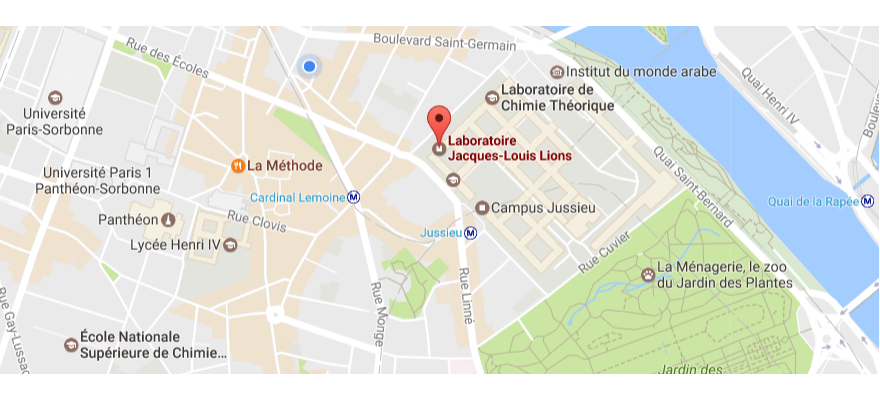
\includegraphics[height=8cm,width=0.9\linewidth]{images/Localisation.png}
\captionof{figure}{Localisation de la structure d'accueil}
\end{center}

%-------------------------------------------------------------------------------------------------------------%
\newpage
\section{Présentation de la problématique du projet}\label{sec:3}

\subsection{Présentation du contexte}\label{sec:3.1}
\hspace{0.5cm}
Afin d'exploiter au mieux son parc nucléaire, la R\&D d'EFD est en train de développer
une nouvelle chaîne de calcul appellée ANDROMEDE, pour simuler le cœur des réacteurs
nucléaires avec des outils à l'état de l'art. L'un des éléments de cette chaîne est le code
neutronique COCAGNE, dont l'un des objectifs est de résoudre numériquement l'équation du
\textbf{transport neutronique} (ou l'une de ses approximations), permettant ainsi d'obtenir des
grandeurs physiques d'intérêt pour décrire le comportement du réacteur, telle que:
le flux neutronique, le facteur de multiplication effectif, la réactivité ... \\
La résolution de cette équation nécessite une grande quantité de données physiques,
en particulier les \textbf{sections efficaces}. \\

En neutronique, les sections efficaces représentent la probabilité d'interaction d'un
neutron incident avec les noyaux cibles, pour différents types d'interaction. Dans une
simulation neutronique, les sections efficaces peuvent être représentées comme des fonctions
dépendant de plusieurs paramètres physiques. Ces paramètres sont utilisés pour décrire les
conditions thermo-hydroliques et la configuration du cœur du réacteur, tel que: la température
du combustible, concentration en bore, niveau de xénon, burnup, ... \\
Ainsi les sections efficaces sont des fonctions multivariées définies sur un espace appelé l'\textbf{espace de phase
des paramètres}. \\

Dans la simulation d'un cœur complet, le nombre de valeurs des sections efficaces est de l'ordre
de plusieurs milliards. Leur détermination demande un calcul complexe et lent.
Pour résoudre ce problème, un schéma en deux étapes est proposé afin de réduire la complexité
des calculs et d'accomplir la simulation du cœur. Ce schéma est basé sur la structure multi-échelle
du noyau du réacteur: noyau contenant des assemblages, assemblages contenant des tiges/cellules (voir figure 2).
\begin{center}
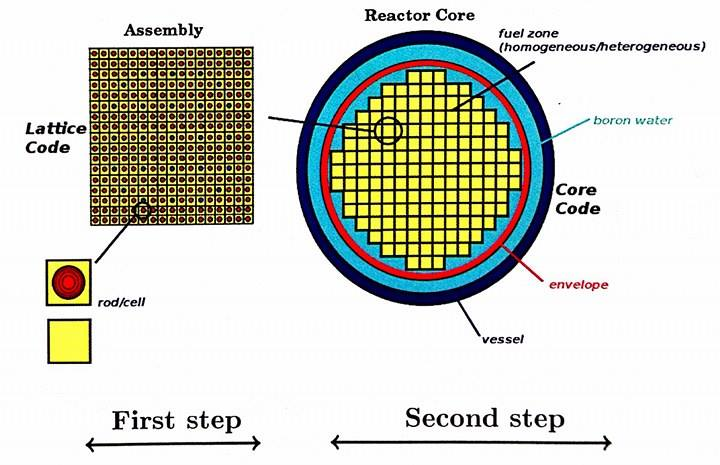
\includegraphics[height=6cm,width=10cm]{images/figure2.jpg}
\captionof{figure}{Schéma à 2 étapes basé sur la structure multi-échelle du noyau du réacteur}
\end{center}

\newpage
Par conséquent, 2 étapes sont effectuées séparément par deux codes:
\begin{itemize}
		\item \textbf{Code réseau:} permet de précalculer les sections efficaces sur des points
		présélectionnés dans l'espace de phase des paramètres (sur chaque assemblage). L'équation du transport neutronique est
		résolue de manière précise grâce à des discrétisations spatiales et énergétique (calcul hors ligne).
		L'information obtenue sur les sections efficaces est stockée dans des fichiers (appelés les \textbf{bibliothèques neutroniques}).
		\item \textbf{Code de cœur:} permet d'évaluer les sections efficaces en n'importe quel point du cœur par interpolation multivariée.
		Les informations stockées dans les biblothèques neutroniques sont utilisées comme données (points d'interpolations)
		pour résoudre l'équation du transport neutronique au niveau du cœur du réacteur.
\end{itemize}
Le schéma ci-dessous (figure 3) illustre le modèle de reconstruction des sections efficaces.
\begin{center}
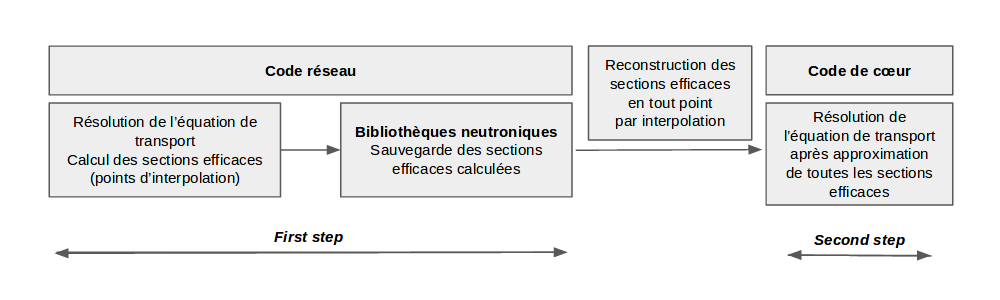
\includegraphics[height=6cm,width=12cm]{images/figure1.png}
\captionof{figure}{Schéma à 2 étapes pour la simulation du cœur du réacteur}
\end{center}

\hspace{0.5cm}
Avec ce modèle, le nombre de points de discrétisation augmente exponentiellement en fonction
du nombre de paramètres ou de manière considérable quand on ajoute des points sur un des axes.
En effet, si on suppose que les sections efficaces dépendent de $d$ paramètres et que chaque
paramètre est discrétisé par $n$ points sur l'axe correspondant, dans ce cas le nombre
de calculs hors ligne et la taille des bibliothèques neutroniques sont de l'ordre de $O(n^d)$.

\newpage
\subsection{Objectifs attendus, problème à résoudre}\label{sec:3.2}
\hspace{0.5cm}
Avec les contraintes industrielles imposées à EDF, le modèle de l'interpolation multivariée
devient très coûteux en mémoire et en temps de calcul pour des situations complexes à cause
de l'augmentation rapide et exponentielle du nombre de points de calcul.
Ces situations peuvent arriver, par exemple, dans le cas accidentel où de nouveaux
paramètres s'ajoutent (température de l'eau, taille des lames d'eau) et/ou quand le domaine
de calcul s'étend (avec des domaines de définition plus larges). \\

Afin de dépasser les limitations de ce modèle, l'objectif de ce stage est de développer
un modèle de reconstitution des sections efficaces tout en répondant aux exigences suivantes:
\begin{itemize}
		\item \textbf{Calculs hors ligne:}
		\begin{itemize}
				\item utiliser moins de précalculs et ceci en choisissant les points de discrétisation de manière astucieuse.
				\item stocker moins de données pour la reconstruction des sections efficaces.
		\end{itemize}

		\item \textbf{Calculs en ligne:} 
		\begin{itemize}
				\item avoir une bonne précision pour l'évaluation des sections efficaces.
		\end{itemize}

\end{itemize}

%-------------------------------------------------------------------------------------------------------------%
\newpage
\section{Solution technique mise en œuvre}\label{sec:4}
\hspace{0.5cm}
Le but de cette partie est de présenter une méthode d'interpolation polynomiale adaptative en grande dimension.
Cette méthode permet d'approximer une fonction multivariée avec une forte précision tout en
utilisant moins de données. \\

Dans la section précédente, on a vu que les sections efficaces sont des fonctions multivariées
définies sur un espace appelé l'espace de phase des paramètres qu'on note $\mathcal{P}$. \\
On peut donc modéliser une section efficace par une fonction $f$ tel que: \\
$f:\mathcal{P} = P^d \rightarrow V_{\Lambda}$ avec $P$ un compact de $\mathbb{R}$ (ou $\mathbb{C}$) et
$V$ l'espace des valeurs prises par les sections efficaces. \\

En pratique, pour $y \in \mathcal{P}$, on peut approcher $f(y)$ avec un code très couteux. Le but est d'éviter ce lent
calcul, tout simplement, en considérant une approximation de $f$ en $y$, qu'on note $\tilde{f}(y)$.
Pour cela, il faut commencer par choisir un certain nombre de point $y^i \in \mathcal{P}, i \in 1..m$. Ensuite on
évalue $f_i = f(y^i) = f(y_1^i, .. , y_d^i)$ en faisant $m$ appel au code couteux. Ensuite, on utilise
$y^1,..,y^m,f_1,..,f_m$ pour fabriquer $\tilde{f}$ par interpolation.\\

L'objectif est donc de construire un opérateur d'interpolation $I_{\Lambda}$ qui permet de reconstruire une
fonction $f$ définie sur $\mathcal{P}$ à valeurs dans $V_{\Lambda}$. \\
Les méthodes d'interpolation polynomiale d'ordre supérieur construisent des approximations de la forme
$u_{\Lambda}(y) = \sum_{\nu \in \Lambda} u_{\nu} y^{\nu}$ avec $\Lambda \in \mathcal{F}$ un ensemble fini de multi-indices
$\nu = (\nu_j)_{j \geq 1} \in \mathcal{F}$ et $y^{\nu} = \prod_{j \geq 1} y_j ^ {\nu_j}$. \\

\textbf{Remarque:}
En dimension finie ($d < \infty$), l'ensemble d'indices $\mathcal{F}$ coincide avec $\mathbb{N}_0^d$.\\
Les $u_{\Lambda}$ sont choisis dans l'espace $V_{\Lambda}$, défini par $V_{\Lambda} = vect \left \{ \sum_{\nu \in \Lambda} v_{\nu} y^{\nu} : v_{\nu} \in V \right \}$

\subsection{Description de la solution envisagée}\label{sec:4.1}
\hspace{0.5cm}
Afin d'approximer $f$ en tout point, on va procéder par interpolation multivariée. Dans cette partie, on va revoir le principe de
l'interpolation de Lagrange en $1D$, puis en dimension quelconque. Par la suite, on évaluera le coût d'une telle opération et son évolution en fonction
du nombre de points d'interpolation et de la dimension de l'espace de phase des paramètres.
Ensuite, on présentera une meilleure méthode d'interpolation adaptative en grande dimension (moins couteuse) basée sur une construction hiérarchique de l'opérateur d'interpolation. \\

\subsubsection{Interpolation monovariée et tensorisation:}\label{sec:4.1.1}
\hspace{0.5cm}
\textbf{ - Cas $d=1$: }
Soit $(y_k)_{k \geq 0}$ une séquence de points deux à deux distincts. \\
On note $I_k$ l'opérateur d'interpolation polynomiale associé à
la séquence $\left \{ y_0, .. , y_k \right \}$. \\
Supposons que la fonction $f$ qu'on veut interpoler est à valeurs dans $\mathbb{R}$ (ou $\mathbb{C}$).\\
\newpage
On a alors,
\begin{align}
   I_k(f) & = \sum_{i=0}^k f(y_i) l_i^k
\end{align}
avec $l_i^k(y) = \prod_{j=0,\ i \neq j}^k \frac{(y - y_j)}{(y_i - y_j)}$, polynômes d'interpolation de Lagrange
de degrès $(k-1)$ associé à la séquence $\left \{ y_0, .. , y_k \right \}$ (voir figure 4). \\
\begin{center}
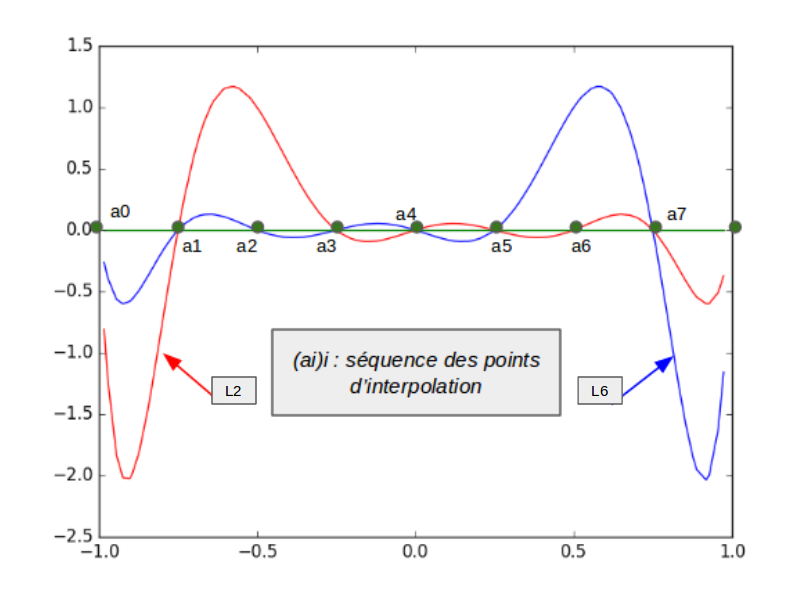
\includegraphics[height=6cm,width=10cm]{images/lagrange_polynomials.png}
\captionof{figure}{Exemples de polynômes d'interpolation de Lagrange}
\end{center}

\vspace{1cm}
\hspace{0.5cm}
\textbf{ - Cas $d>1$: }
On procède par tensorisation. \\
C'est à dire, pour $\alpha_1,..,\alpha_d \in \left \{0,.., k-1 \right \}$ \\
\begin{align}
   \tilde{f} (y_1,..,y_d)& = \bigotimes_{i=1}^d I_k (f)(y_1,..,y_d) \in \mathbb{Q}_{k-1} = vect \left \{ y \rightarrow y_1^{\alpha_1}..y_d^{\alpha_d} \right \} \\
	 & = \sum_{k_1=1}^k..\sum_{k_d=1}^k (f(y_{k_1},..,y_{k_d}) l_{k_1}(y_1)..l_{k_d}(y_d))
\end{align}
\hspace{0.5cm}
Pour avoir une bonne précision, il est préférable de choisir un nombre relativement grand de points d'interpolation.
Si par exemple, on prend $k_j$ points suivant la direction $j$, on obtient un nombre total de points égal à $\prod_{i=1}^d k_j$.
Ceci pose problème, bien évidemment, lorsque $d$ est grand. En effet, non seulement le calcul de $\tilde{f}$ sera couteux, mais aussi,
si on souhaite ajouter $1$ points suivant la variable $i$ ça revient à ajouter $\prod_{j=1,\\ j \neq i}^d k_j$ nœuds dans la grille (voir figure 5).\\
\begin{center}
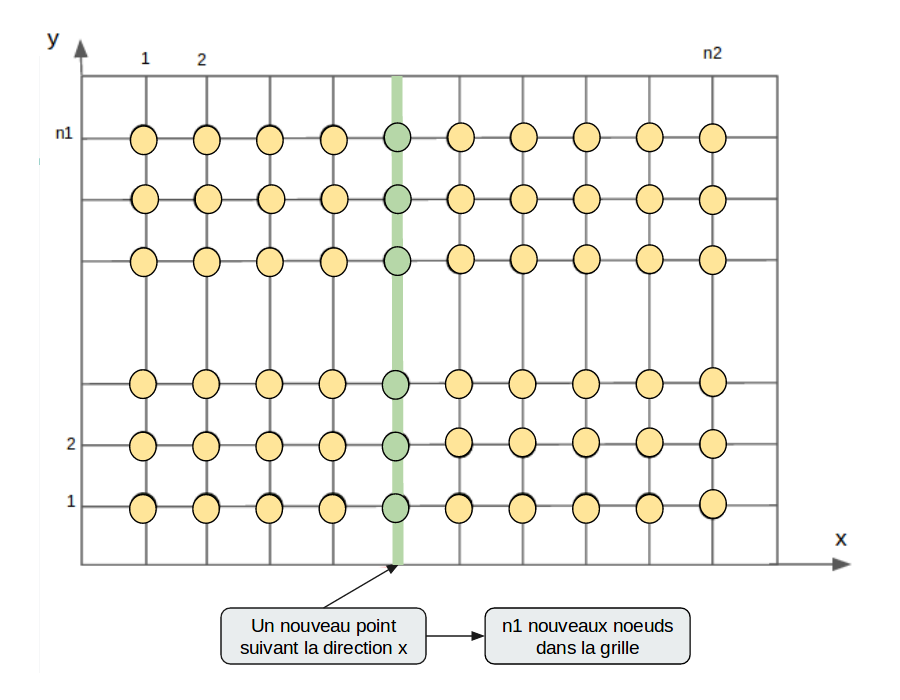
\includegraphics[height=9cm,width=12cm]{images/grille.png}
\captionof{figure}{Influence de l'ajout d'un point d'interpolation sur une seule direction}
\end{center}

Cette méthode d'interpolation devient très coûteuse lorsqu'il s'agit de fonctions multivariées en grande dimension.\\
Une solution serait de calculer l'opérateur d'interpolation par une méthode hiérarchique. C'est à dire qu'on va
utiliser les approximations de $f$ à l'ordre $j<k$ ($I_{j}(f)$ obtenue avec $j$ points d'interpolation) pour approcher $I_{k}(f)$.

\subsubsection{Construction hiérarchique de l'opérateur d'interpolation:}\label{sec:4.1.2}
\hspace{0.5cm}
\textbf{ - Cas $d=1$: }
Soit $k \geq 0$, on définit l'opérateur différence $\Delta_k$ par:
\begin{align}
   \Delta_k & =  I_k - I_{k-1}
\end{align}
On suppose, par convention, que $I_{-1}$ est l'opérateur nul. De cette façon, $I_0 = \Delta_0$ correspond à
l'opérateur qui à $f$ associe le polynôme constant $f(y_0)$.\\
On a alors,
\begin{align}
   I_n & = \sum_{k=0}^n \Delta_k
\end{align}
On définit ensuite, les polynômes hiérarchiques de degré $k$ associés à la séquence $\left \{ y_0, .. , y_k \right \}$ par
\begin{align}
	 h_k(y) & = \prod_{j=0}^{k-1} \frac{(y - y_j)}{(y_k - y_j)}, k > 0,\ et\ h_0(y) = 1,
\end{align}
On a alors,
\begin{align}
	\Delta_k(f) & = \alpha_k(f)h_k, \ \ \ \alpha_k(f) = f(y_k) - I_{k-1} f(y_k)
\end{align}
On obtient alors, par un processus itératif, la représentation suivante:
\begin{align}
   I_n(f) & = \sum_{k=0}^n \alpha_k(f)h_k
\end{align}
Ainsi pour calculer l'interpolant de $f$ en utilisant $n$ points, il suffit de connaître les intérpolants de $f$ d'ordre $i$,
$i \in \left \{1,..,n-1 \right \}$, et ceci d'une manière relativement rapide. \\

\hspace{0.5cm}
\textbf{ - Cas $d>1$: }
On veut effectuer une interpolation polynomiale pour une séquence imbriquée d'ensemble $(\Lambda_n)_{n \geq 1}$ avec $n=\sharp(\Lambda_n)$. \\
Pour la suite, on définit :
\begin{itemize}
		\item Le point multivarié $\textbf{y}_{\nu}$ par $\textbf{y}_{\nu} = (y_{\nu_j})_{j \geq 1} \in \mathcal{P}$
		\item La fonction polynomiale hiérarchique tensorisée $\textbf{H}_{\nu}$ par $\textbf{H}_{\nu}(y) = \prod_{j \geq 1} h_{\nu_j} (y_j)$
\end{itemize}
		Pour que la méthode décrite précedament en $1D$ fonctionne en dimension $d>1$, il faut s'assurer que pour tout $n \geq 1,\ \Lambda_n$ est monotone. \\

\fbox{\begin{minipage}{0.9\textwidth}
\textbf{Définition: }Un ensemble $\Lambda \subset \mathcal{F}$, non vide, est dit monotone, si
\begin{align}
  	& \nu \in \Lambda \ et\ \mu < \nu \Rightarrow \mu \in \Lambda
\end{align}
\hspace{2cm} avec $\mu \leq \nu$ signifie que $\mu_j \leq \nu_j$ pour tout $j$. \\
\end{minipage}}

\vspace{0.5cm}
Dans cette configuration, $\Lambda_n$ peut être vu comme une section $\left \{ \nu^1, .. , \nu^n \right \}$ d'une séquence
$(\nu^k)_{k \geq 1} \in \Lambda^{\mathbb{N}}$. Cette observation mène à un algorithme efficace pour le calcul de
$I_{\Lambda_n}f$ à partir de $I_{\Lambda_{n-1}}f$ et de la valeur de $f$ en le nouveau point $\textbf{y}_{\nu^n}$. En effet,
on remarque que $\Delta_{\nu^n}$ est multiple de la fonction hiérarchique tensorisée $\textbf{H}_{\nu^n}$ défini précedement.\\
Puisque $\textbf{H}_{\nu^n}(\textbf{y}_{\nu^n}) = 1$, alors \\
\begin{align}
	 \Delta_{\nu^n}f &= \Delta_{\nu^n} f(\textbf{y}_{\nu^n}) \textbf{H}_{\nu^n} \\
	 &= (I_{\Lambda_n}f(\textbf{y}_{\nu^n}) - I_{\Lambda_{n-1}}f(\textbf{y}_{\nu^n})) \textbf{H}_{\nu^n} \\
	 &= (f(\textbf{y}_{\nu^n}) - I_{\Lambda_{n-1}}f(\textbf{y}_{\nu^n})) \textbf{H}_{\nu^n}
\end{align}
Donc
\begin{align}
	 I_{\Lambda_n}f & = I_{\Lambda_{n-1}}f + (f(\textbf{y}_{\nu^n}) - I_{\Lambda_{n-1}}f(\textbf{y}_{\nu^n})) \textbf{H}_{\nu^n}
\end{align}
Par conséquent, les polynômes $I_{\Lambda_n}f$ sont donnés par:
\begin{align}
	 I_{\Lambda_n}f & = \sum_{k=0}^n f_{\nu^k} \textbf{H}_{\nu^k}
\end{align}
avec $f_{\nu^k}$ définis récursivement par:
\begin{align}
	 f_{\nu^1} & = f(y_0),\ \ f_{\nu^{k+1}} = f(\textbf{y}_{\nu^{k+1}}) - I_{\Lambda_{k}}f(\textbf{y}_{\nu^{k+1}}) = f(\textbf{y}_{\nu^{k+1}}) - \sum_{i=1}^k f_{\nu^i} \textbf{H}_{\nu^i}(\textbf{y}_{\nu^{k+1}})
\end{align}

\newpage
\subsubsection{Interpolation adaptative et séquence de points d'interpolation:}

\hspace{0.5cm}
Les ensembles $\Lambda_n$ peuvent être choisis préalablement de sorte qu'ils forment une
séquence imbriquée d'ensembles monotones. Ils peuvent aussi être construits d'une manière astucieuse
lors du calcul de l'interpolant en construisant un chemin qui correspond à un ordre entre les points d'interpolations. \\

Soit l'analogie suivante: si $(\textbf{H}_{\nu})_{\nu \in \mathcal{F}}$ est une base orthoromée de $L^2(\mathcal{P})$ alors
le choix d'un ensemble d'indices $\Lambda_n$ qui minimise l'erreur  serait de prendre les $n$ plus grands $a_{\nu} \left | f_{\nu}  \right |$
tel que $a_{\nu} = \left \| \textbf{H}_{\nu} \right \|_{L^{\infty}(\mathcal{P})} = \prod_{j \geq 1} \left \| {h_{\nu_j}} \right \|_{L^{\infty}(\mathcal{P})}$. \\
Cette stratégie permet d'avoir une séquence imbriquée $(\Lambda_n)_{n \geq 1}$, cependant il n'est pas certain que les
ensembles $\Lambda_n$ soient monotones. \\
Afin de résoudre ce problème, on définit la notion de voisins pour n'importe quel ensemble monotone $\Lambda$ par,
\begin{align}
	 \mathcal{N}(\Lambda) & = \left \{ \nu \notin \Lambda : R_{\nu} \in \Lambda \cup \left \{ \nu \right \} \right \}, R_{\nu} = \left \{ \mu \in \Lambda : \mu < \nu \right \}
\end{align}
Ainsi, avec cette définition, l'algorithme ci-dessous mène à une séquence imbriquée d'ensembles monotones. \\

\textbf{Algorithme d'Interpolation Adaptative:}

\vspace{0.5cm}
\fbox{\begin{minipage}{0.9\textwidth}
\begin{itemize}
\item Commencer par $\Lambda_1 = \left \{0_{\Lambda} \right \}$
\item En supposant $\Lambda_{n-1}$ calculé, trouver $\nu^n = argmax \left \{ a_{\nu} \left | f_{\nu} \right | : \nu \in \mathcal{N}(\Lambda_{n-1}) \right \}$, et définir $\Lambda_n = \Lambda_{n-1} \cup \left \{ \nu \right \}$
\end{itemize}
\end{minipage}}

\vspace{0.5cm}

Il est important de noter que le choix de la séquence de points d'interpolation joue un rôle critique
pour la stabilité de l'opérateur d'interpolation multivariée définie par la constante de Lebesgue:
\begin{align}
		\mathbb{L}_{\Lambda} = sup_{f \in B(\mathcal{P})-{0}} \frac{\left \| I_{\Lambda}f \right \|_{L^{\infty}(\mathcal{P})}}{\left \|f \right \|_{L^{\infty}(\mathcal{P})}}
\end{align}
avec $B(\mathcal{P})$ est l'espace des fonction bornées définis sur $\mathcal{P}$\\
L'objectif est de choisir la séquence $(y_k)_{k \geq 0}$ tel que les constantes monovariées de Lebesgue
\begin{align}
		\lambda_k & = max_{f \in B(\mathcal{P})-{0}} \frac{\left \| I_k f \right \|_{L^{\infty}(\mathcal{P})}}{\left \|f \right \|_{L^{\infty}(\mathcal{P})}}
\end{align}
associées à l'opérateur d'interpolation monovariée $I_k$ croient modérément par rapport à k.
Une telle séquence peut être construite en fixant $y_0 \in P$ et en définissant inductivement
\begin{align}
		y_k & = argmax_{y \in P} \prod_{j=0}^{k-1} \left | y - y_j \right |
\end{align}
Cette séquence $(y_k)_{k \geq 0}$ est appellée séquence de Leja \cite{Leja} sur P. Elle modère la croissance des constantes de Lebesgue
et a une implication intéressante sur le choix adaptatif des $\Lambda_n$.\\
Voici les $10$ premiers points de la séquence de Leja construite dans l'intervalle $\left [ -1, 1 \right ]$ :
\begin{align}
\left \{\ 1,\ -1,\ 0,\ -0.577316,\ 0.658716,\ -0.83924,\ 0.870029,\ 0.305729,\ -0.321539,\ -0.942991\ \right \} \nonumber
\end{align}

\hspace{0.5cm}La précision de l'interpolation dépend fortement du choix des fonctions hiérarchiques de base et de la séquence des points d'interpolation.
Quand il s'agit d'approcher des fonctions plates ou polynomiales de n'importe quel ordre, il est intéressant de choisir les polynômes hiérarchiques de Lagrange ainsi que la séquence de Leja.\\
En effet, non seulement, on obtient l'interpolant au bout d'un nombre d'itérations relativement petit, mais aussi avec une grande précision.

\hspace{0.5cm}Cependant, quand il s'agit d'approcher des fonctions plus complexes, par exemple des fonctions présentant de fortes variations brusques, ou certaines irrégularités, le choix précedant n'est
plus intéressant.\\

\hspace{0.5cm}On a vu que l'algorithme AI évolue en localisant les points où l'erreur d'interpolation est la plus élevée. Parfois, il est très difficile de détécter
un point où l'erreur est grande. Pour mieux voir cela, considérons l'exemple de la figure ci-dessous. \\
Cette figure est divisé en deux parties. Chaque partie correspond à une itération particulière dans l'algorithme AI.\\
Chaque partie est divisée verticalement en deux graphes:
\begin{itemize}
\item Celui en haut montre l'interpolé (en vert) et l'interpolant (en rouge).
\item Celui en bas montre les fonctions de bases construites jusqu'à l'itération courante.
\end{itemize}
\begin{center}
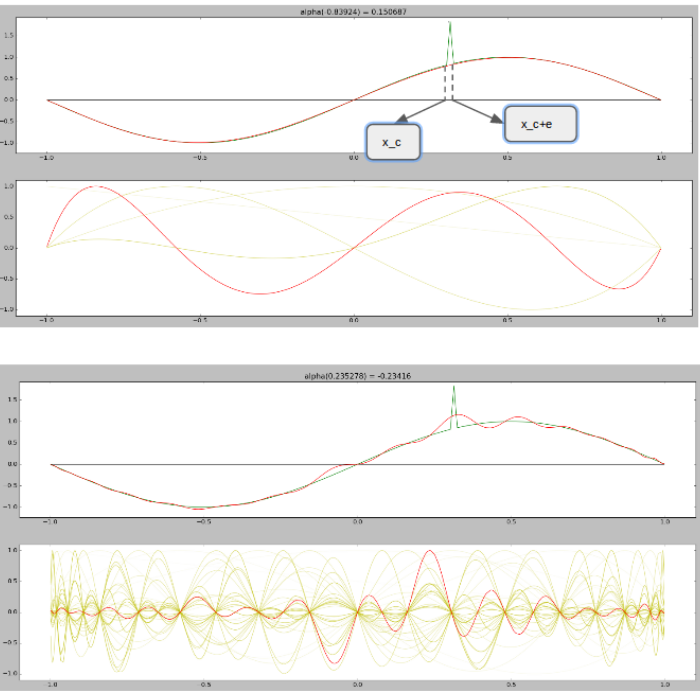
\includegraphics[height= 11cm,width = 11cm]{images/lag_glob.png}
\captionof{figure}{Interpolation utilisant des polynomes de Lagrange définis globalement}
\end{center}
\newpage
Dès qu'un nouveau point d'interpolation est ajouté dans l'intervalle $ \left [ x_c, x_c+\epsilon \right ]$, on obtient des perturbations de l'interpolant ailleurs.
Ce qui provoque une augmentation concidérable de l'erreur. Ceci est dû au caractère global des fonctions hiérarchiques.\\

\hspace{0.5cm}Dans de telles situations il est plus judicieux d'utiliser des fonctions polynômiales par morceaux comme fonctions hiérarchiques de base.\\
De cette façon, chaque nouveau point d'interpolation ajouté, ne provoque que des perturbations locales, ce qui ne dégrade pas trop l'interpolation obtenu jusque là.\\
Dans ce cas de figure, on choisit un nouveau type de points d'interpolation qui est mieux adéquat. La séquence sera formée par un ensemble de points obtenu en discrétisant pogréssivement
le domaine par dichotomie.\\
Voici, un exemple en 1D pour mieux comprendre cela.\\
Supposons que $P = \left [ -1, 1 \right ]$ et que le premier point d'interpolation est $0$. Alors, la séquence de points d'interpolation évoluera
de la façcon suivante.\\
On suppose que $S$ est la séquence de points d'interpolation, et $V$ la liste courante des points voisins de $S$.
\begin{itemize}
\item \textbf{Iteration 0:} $S = \left \{ 0 \right \}$ et $V = \left \{ -1,1 \right \}$
\item \textbf{Iteration 1:} ($S = \left \{ 0, -1 \right \}$ et $V = \left \{ 1, -0.5 \right \}$) ou \\
($S = \left \{ 0, 1 \right \}$ et $V = \left \{ 1, 0.5 \right \}$)
\item \textbf{Iteration 2:} ($S = \left \{ 0, -1, 1\right \}$ et $V = \left \{ -0.5, 0.5 \right \}$) ou \\
($S = \left \{ 0, -1, -0.5 \right \}$ et $V = \left \{ 1, -0.25, -0.75\right \}$) ou \\
($S = \left \{ 0, 1, -1 \right \}$ et $V = \left \{ -0.5, 0.5\right \}$) ou \\
($S = \left \{ 0, 1, 0.5 \right \}$ et $V = \left \{ -1, 0.25, 0.75\right \}$)
\end{itemize}
En d'autres termes, le nouveau point d'interpolation sera celui, parmi les voisins de $S$ (courant), au niveau duquel l'erreur d'interpolation est maximale.
Ce point appartient forcement à l'ensemble des nœuds descendant directement des points de $S$ dans l'arbre ci-dessous.
\begin{center}
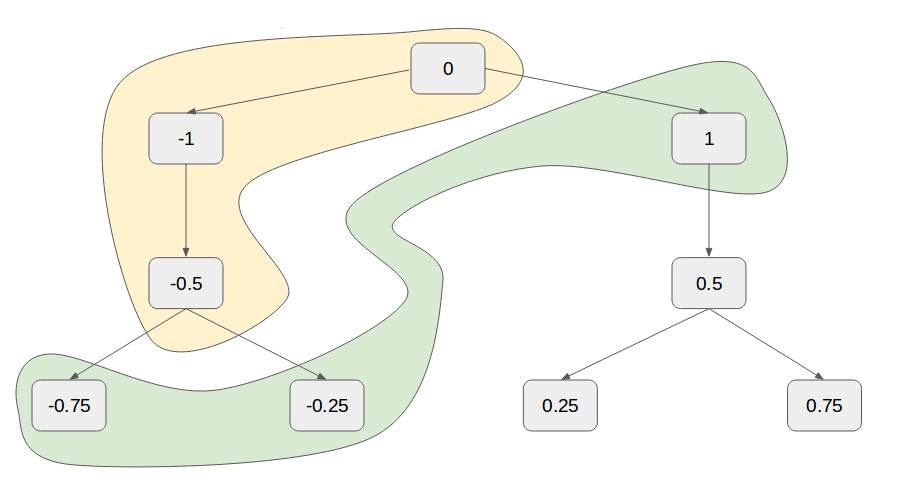
\includegraphics[height= 6 cm,width = 9 cm]{images/tree.png}
\captionof{figure}{Arbre représentatif des points d'interpolation en 1D}
\end{center}
Dans la figure précedante, l'ensemble jaune correspond à la séquence d'interpolation, et celui en vert correspond à l'ensemble courant des points voisins.\\
Etant donné qu'on a besoin d'une notion d'ordre entre les points d'interpolation, on introduit la relation suivante: un nœud $n$ est d'ordre plus élevé qu'un nœud $m$ si et seulement si $m$ est un ancêtre de $n$.\\
Ainsi, en grande dimension, et avec ce type de séquence, on est capable de définir un ensemble monotone vu qu'on a une relation d'ordre entre les nœuds.
La figure ci-dessous, montre le résultat de l'interpolation d'une fonction de même type que précedement, cette fois, en utilisant des fonctions quadratique par morceaux comme fonctions de base.\\
On remarque que dès que l'algorithme détecte un point dans la zone critique, il corrige l'interpolant courant sans pour autant provoquer des erreurs ailleurs.\\
\begin{center}
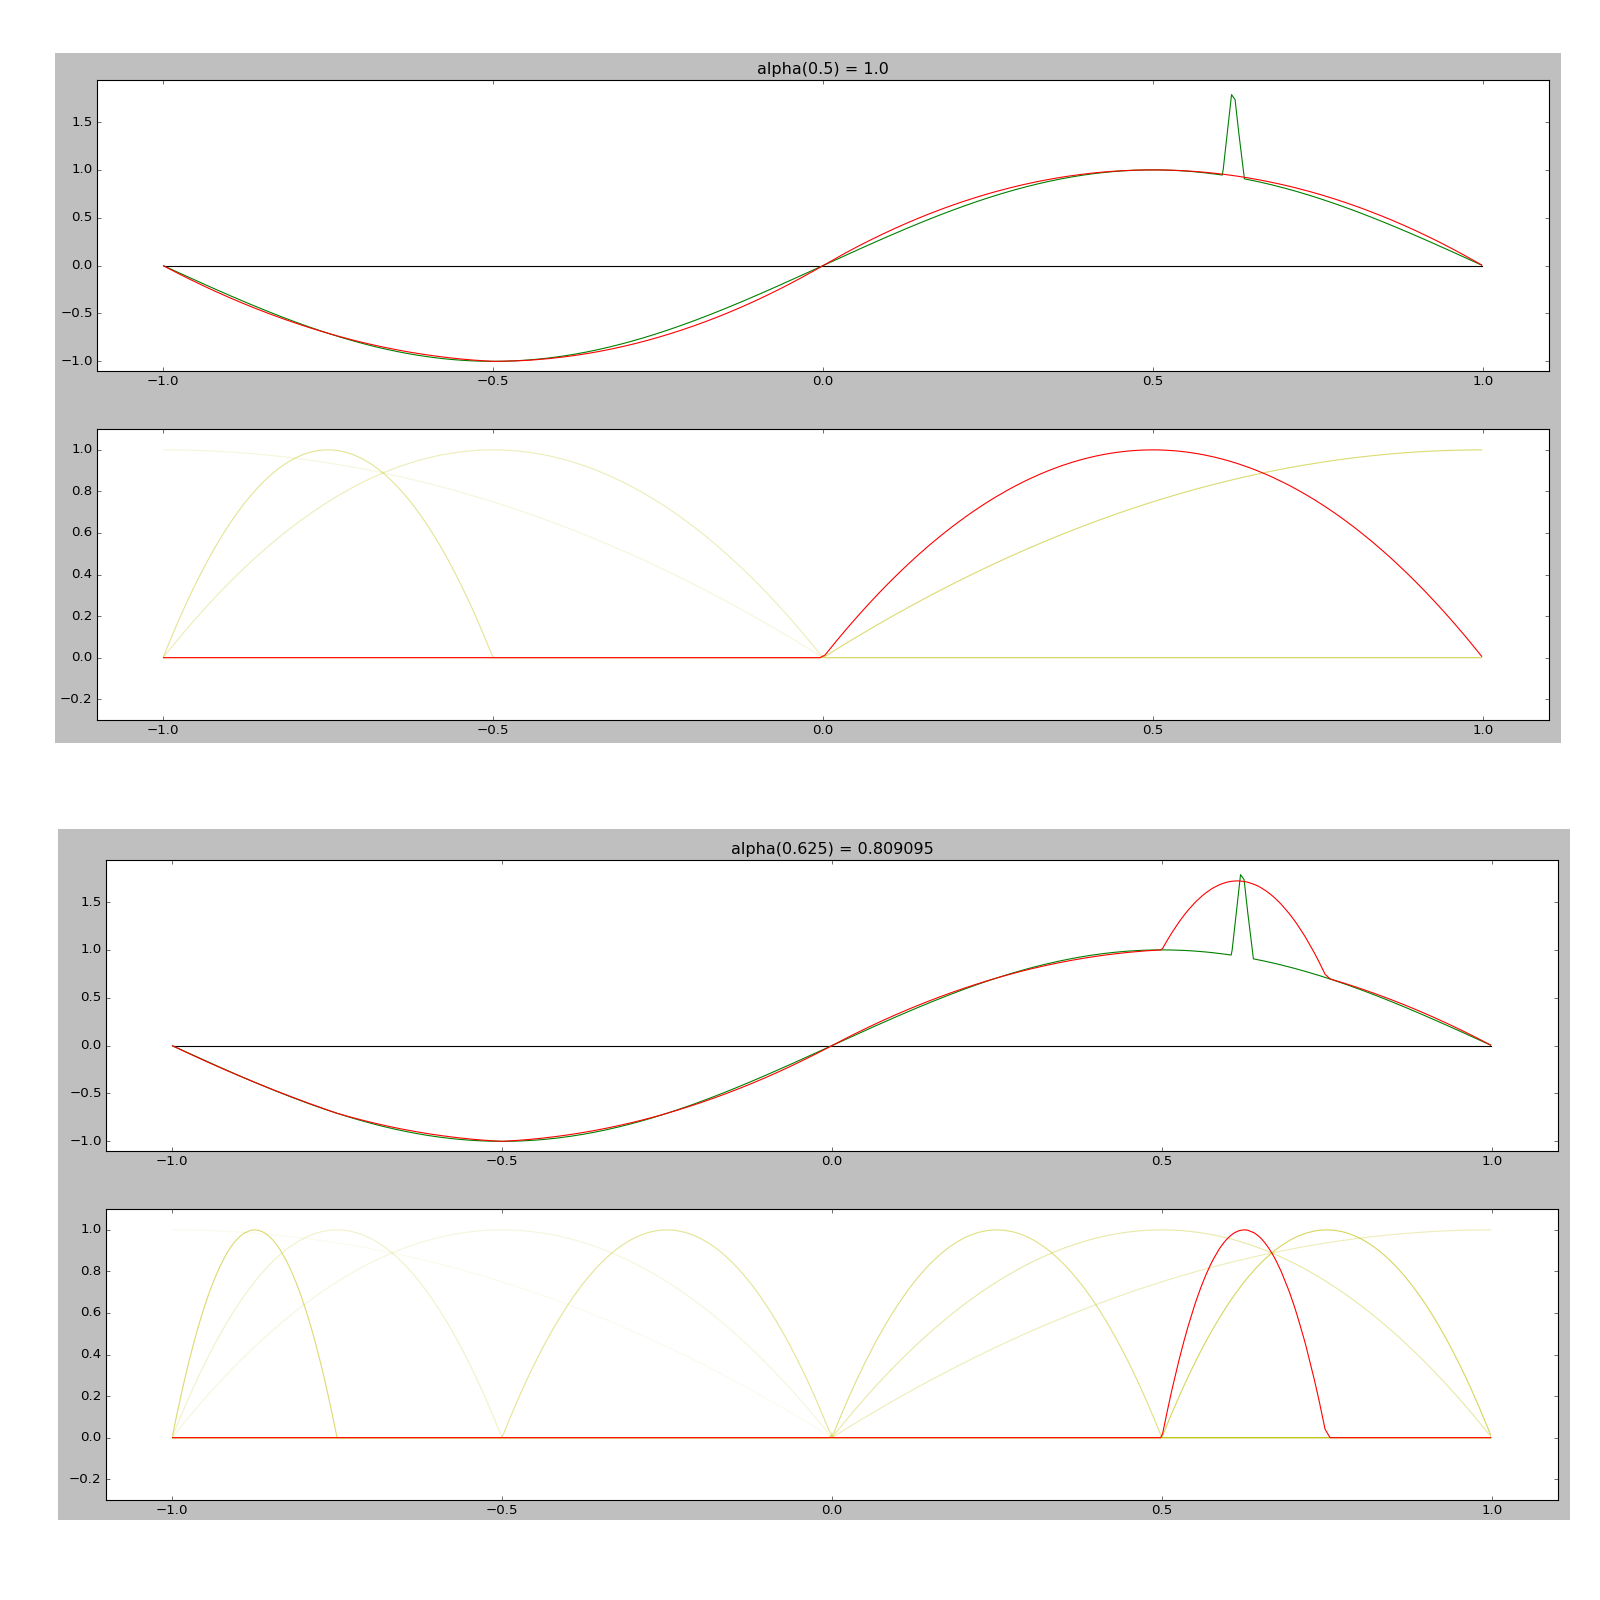
\includegraphics[height= 11cm,width = 11cm]{images/interp_pm.png}
\captionof{figure}{Interpolation utilisant des fonctions quadratiques par morceaux}
\end{center}

\textbf{Remarque:}
\begin{itemize}
\item Certains nœuds ne peuvent être comparés (exemple $-1$ et $0.5$) car l'un n'est ni ancêtre, ni descendant de l'autre.\\
\item En 1D, et pour une itération $(i>0)$ le nombre de voisins (éventuels futur points d'interpolation) obtenu avec la méthode d'interpolation par polynômes de Lagrange est inférieur
à celui obtenu en utilisant des fonctions quadratique par morceaux. \\
En effet, avec la première méthode, on a toujours un seul voisin possible (qui correspond au point suivant dans la séquence de Leja).
Par contre, avec l'autre méthode, on en a plus car il y a toujours 2 voisins pour chaque point (qui correspondent au nœuds filles dans l'arbre) sauf pour les extrémités ($-1$ et $1$).
\item La méthode d'interpolation par fonctions quadratiques (ou affines) par morceaux n'est pas toujours meilleure que celle par polynômes de Lagrange.
Le cas le plus évident est quand l'interpolé est un polynome. Dans ce cas, on obtient une bonne approximation avec les deux méthodes.
Sauf qu'avec la méthode utilisant les polynômes de Lagrange, l'algorithme est beaucoup plus précis et rapide (car il y a toujours moins de voisins à évaluer).
\item En dimension quelconque on peut avoir des fonctions ayant une nature différente suivant chaque variable. Dans ce cas, il est possible de combiner les deux méthodes.
En effet, considérons la fonction $f : (x,y) \rightarrow \sqrt{1-x^2}\exp(y)$.
La meilleure façon d'interpoler $f$ est d'utiliser des fonctions quadratiques par morceaux selon la direction x et des polynômes de Lagrange suivant la direction y.
\end{itemize}



\subsection{Implèmentation de la solution}\label{sec:5}
Dans cette partie, on va mettre en pratique cette méthode et on va présenter certains détails
de l'implémentation de cette solution (notamment la construction de la séquence des points d'interpolation).\\
Cette solution a été implémenté en C++. Le code est constitué principalement des classes suivantes:

\begin{itemize}
\item \textbf{Classe Interpolation<T>:} Il s'agit d'une classe générique abstraite. Elle implémente les structures de données contenants les différentes quantités qui entrent
en jeu dans la construction de l'opérateur d'interpolation, notamment les points d'interpolations, les points de test,
la liste des voisins courants dans l'algorithme AI, et le chemin d'indices vu dans la section précédente. De plus, l'algorithme AI ainsi que certaines fonctions intermédiaires,
(notamment celle responsable de la recherche des voisins dans une grille) sont implémentés dans la classe $Interpolation<T>$.
Ici, $T$ fait référence au type données utilisé pour représenter l'ordre des points d'interpolation. Vu qu'il est différent pour les deux méthodes, on a choisi de procéder par généricité.\\
Cependant, il y a plusieurs similarité entre les deux méthodes, d'où le choix d'implémenter une classe abstraite, ensuite de faire deux classes filles qui héritent des fonctionnalitées communes.

\item \textbf{Classe LagrangeInterpolation:} Cette classe hèrite de Interpolation<int> et elle implémente la méthode utilisant les polynômes de Lagrange.

\item \textbf{Classe PiecewiseInterpolation:} Cette classe hèrite de Interpolation<string> et elle implémente la méthode utilisant les polynômes de Lagrange.

\item \textbf{Classe MixedInterpolation:} Cette classe hèrite de Interpolation<string> et elle implémente une combinaison des 2 méthode. Ici, on utilise des chaînes de caractère
car, avec ce type de donnée, on peut à la fois représenter les codes de Huffman ainsi que de simples entiers.

\item \textbf{Classe BinaryTree:} Cette classe implémente un arbre binaire qui permet de coder les points cartésiens et les ordonner.
Cette classe est utile dans la version de l'algorithme AI qui utilise des fonctions de bases quadratiques par morceaux.
En effet, on ne peut pas ordonner les points d'interpolation par des indices comme dans l'autre méthode (chaque indice correspond à l'ordre du réel dans la séquence de Leja).\\

Cependant, on a besoin de fonctionnalitées qui nous permettent de situer un point d'interpolation parmi d'autres ou de retrouver les deux points les plus proches pour pouvoir construire la fonction
de base correspondante. L'idée ici est de coder chaque point, non par un indice mais par une chaîne de caractère qui n'est autre que le code de Huffman correspondant dans l'arbre.
Ainsi, on est capable de définir une méthode pour comparer l'ordre des points. Chaque arbre est construit de la façon suivante:
\begin{itemize}
\item Le point $0.0$ est la racine.
\item Chaque nœud possède au maximum 2 fils.
\item Les points $-1.0$ et $1.0$ (extrémités du $P$) possédent chacun exactement un fils.
\item Soit $n$ un noeud intermédiare, on note $p$ son père, $g$ son fils gauche, et $d$ son fils droite, on a alors:
\begin{align}
g =
\begin{cases}
 -1 & \text{ si } n=0 \\
 n-\left | p-n \right |/2 & \text{ si } n\neq0
\end{cases}
\\
d =
\begin{cases}
 -1 & \text{ si } n=0 \\
 n+\left | p-n \right |/2 & \text{ si } n\neq0
\end{cases}
\end{align}
\end{itemize}
Le code de chaque nœud $n$ est construit en parcourant l'arbre de la racine jusqu'au point $n$.
Le code est initialement une chaine vide. Chaque fois qu'on va à gauche (resp à droite) ou écrit $0$ (resp $1$).\\
Ainsi le code de $-0.375$ dans l'arbre ci-dessous est $"0110"$.\\
\begin{center}
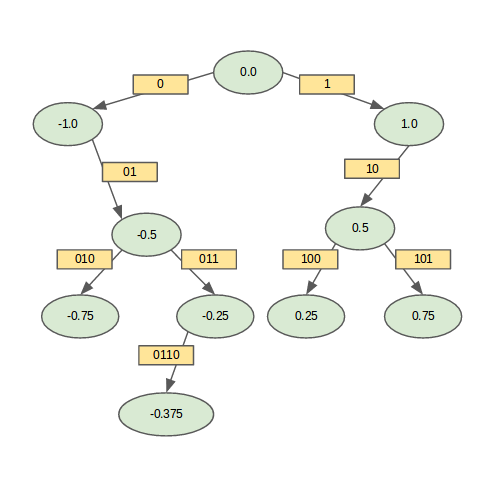
\includegraphics[height= 11cm,width = 11cm]{images/huffman.png}
\captionof{figure}{Codage de huffman de chaque nœud de l'arbre}
\end{center}
Avec ce codage, on est capable de retrouver facilement, à partir de d'un nœud $n$ le code de son parent ou encore des nœuds ayant les valeurs les plus proches.\\

\item \textbf{Classe MultivariatePoint<T>:} Il s'agit d'une classe générique qui modélise à la fois les multi-indices, ainsi que les points réels multivariés.
C'est à dire qu'une instance de cette classe peut renfermer soit des valeurs réelles, soit des entiers, soit des chaînes de caractères qui correspondent aux codes de Huffman
du point réel en question.\\
Les opérateurs d'affectation, d'addition, d'affichage ainsi que de comparaison de points multivariés sont implémentés dans cette classe.
Un multi-indice correspond à un ensemble d'ordres. Par exemple: en 2D, le vecteur $(0,1) \in \mathbb{N}^2$ correspond au point $(1.0,-1.0) \in \mathcal{P}$. \\
En effet, $1.0$ (resp $-1.0$) étant le point d'indice $0$ (resp $1$) dans la séquence de Leja.\\
Par contre, quand il s'agit d'utiliser une séquence de points construits par dichotomie, on utilisera des chaînes de caractères. Par exemple : en 2D,
le vecteur $("","01")$ correspond au point $(0,-0.5) \in \mathcal{P}$.\\

\item \textbf{Classe Utils:} Il s'agit d'une classe statique renfermant certaines fonctions utiles notamment les fonctions d'affichages,
les fonctions qui gèrent la création des séquences d'interpolations (notamment la séquence uniforme, les zéros de Tchebychev ainsi que la séquence de Leja).
De plus, cette classe permet de lire des donnée et d'écrire les résultats dans des fichiers externes.

\item \textbf{Classe Functions:}
Cette classe implémente certaines fonctions analytiques qui permettront de tester l'algorithme d'Interpolation Adaptative. De plus, elle permet de lire et d'organiser
et d'intégrer les données réelles fournies par le département R\&D d'EDF.
\end{itemize}

\paragraph{Construction de la séquence de Leja:}
L'idée est de discrétiser l'intervalle de définition $U$ de la fonction $f$ en un grand nombre de points $(a_i)_{i=1..n(=100000)}$.
Supposons qu'on a construit à l'étape $i$ la séquence $\left \{ y_0,..,y_i \right \}$, alors pour avoir le point $y_{i+1}$,
on compare le produit des distances de chaque point de discrétisation aux points de Leja déja calculés, puis on choisit le max.\\
La façon la plus naturelle de choisir les points $a_i$ est de les choisir uniformément répartis dans l'intervalle de définition de $f$.\\
On obtient alors une suite de polynômes qui interpole $f$ en de plus en plus de points. On pourrait s'attendre à ce que la suite converge
uniformément vers $f$ lorsque le nombre de points d'interpolation augmente.\\
Malheureusement, ce n'est pas le cas, ce phénomène est connu sous le nom de phénomène de Runge. \\
Une solution est, étonnamment, de ne pas choisir les points uniformément répartis. Une raison pour cela est l'inégalité suivante :
si $f$ est de classe $C^N$ sur l'intervalle $U$ et si $L$ est le polynôme d'interpolation de Lagrange en les points $a_1,..,a_N$, alors on a
\begin{align}
		& \forall x \in U, \left |f(x)-L(x)\right | \leq sup_{x \in U}  (\prod_{i=1}^n \left | x-a_i \right |) \frac{\left \|f^{(n)} \right \|_{\infty}}{n!}
\end{align}
\hspace{0.5cm}
L'idée est donc de choisir les $a_i$ de sorte que $sup_{x \in U}  \prod_{i=1}^n \left | x-a_i \right |$ soit le plus petit possible. On démontre que
ceci est réalisé lorsque les $a_i$ sont les zéros du polynôme de Tchebychev de degré $n$, à savoir $a_i = cos(\frac{(2i-1) \pi}{n}), i =1,..,n$.\\
La figure 6 montre une grille 2D formés par des points de Leja construits dans le segment $\left [-1,1 \right ]$.\\
\begin{center}
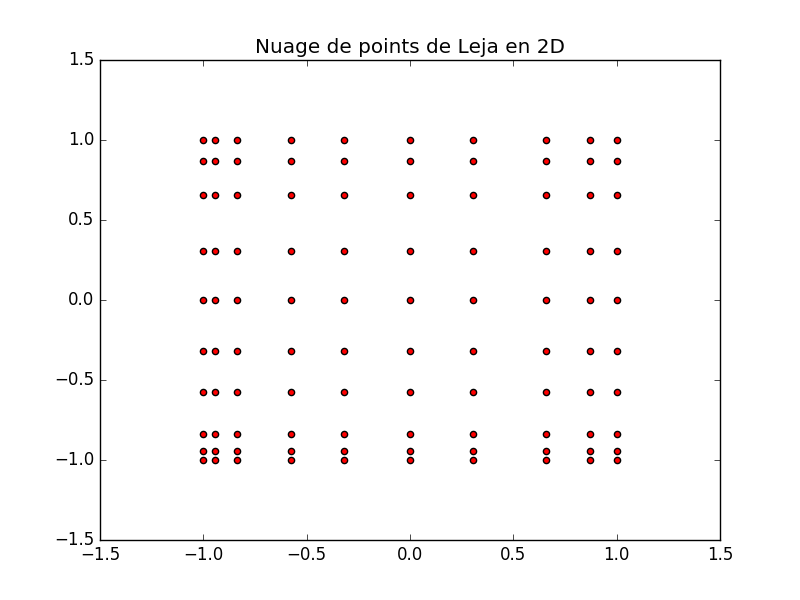
\includegraphics[height= 9 cm,width = \linewidth]{images/leja_sequence.png}
\captionof{figure}{Grille 2D des points de Leja}
\end{center}

\section{Évaluation de l’efficacité de la méthode}\label{sec:6}
L'algorithme d'Interpolation Adaptative a été tésté avec des fonctions analytiques définies à l'avance en des points choisis d'une manière aléatoire.\\
Les résultat obtenus ont été ensuite comparé à ceux obtenus avec une autre méthode d'approximation de fonctions multivariées basée sur
le modèle de décomposition de Tucker.\\
L'étape suivante a été de tester les deux méthodes sur des données réelles fournies par le département R\&D d'EDF et de les comparer.

\subsection{Présentation du modèle de décomposition de Tucker}
\subsection{Tests et comparaisons}
\subsubsection{Fonctions analytiques prédéfinies}
\subsubsection{Données réelles}
Le cœur d'un réacteur nucléaire posséde une structure multi-échelle. Il contient entre 150-200 assemblages combustibles disposés en treillis carré
et entourés d'eau de bore. Un assemblage typique est souvent constitué de $17x17=289$ tiges, dont 264 tiges de carburant et 25 tiges vides.
Il existe plusieurs types d'assemblages selon la position et la composition des tiges de carburant.
\begin{itemize}
\item \textbf{Assemblage UOX (Uranium Oxide: $UO_2$):}
\item \textbf{Assemblage MOX (Mixed Oxide: $UO_2-PuO_2$):}
\item \textbf{Assemblage UOX-Gd (UOX-Gadolinium: $UO_2-Gd_2O_3$):}
\end{itemize}

\subsection{Conclusion et remarques}

%-------------------------------------------------------------------------------------------------------------%
\section{Impressions personnelles}\label{sec:7}
\hspace{0.5cm}
Au début du stage et notamment au cours des premières présentations du sujet, ce dernier m'a paru
plutôt difficile. Il m'a fallu une certaine période de documentation et de recherche avant de pouvoir entamer la partie pratique.
Ainsi, au bout des premières semaines de mon stage, j'ai réussi à bien assimiler la partie théorique du sujet.
Ce sujet m'a paru alors encore plus intéressant car j'ai pu constater sa richesse en matière de spectre d'applications. De plus j'ai eu l'occasion
de beaucoup apprendre notamment sur l'interpolation en grande dimension en général, mais aussi au niveau de la programmation informatique. En effet, j'ai
pu améliorer mes connaissances en python et mettre en application tout ce que j'ai appris en algorithmique et en C++.\\

De plus, étant donnée que mes encadrants ont participé à l'étude et la réalisation de la partie théorique, il m'était facile d'évoluer
et d'avancer dans ma compréhension des différents points-clés de mon sujet de stage. En effet, le fait qu'ils soient souvent disponibles
pour discuter des points potentiellement imprécis et de l'organisation du travail m'a évité une importante perte de temps.\\
Par ailleurs, j'ai été agréablement surpris par l'environnement et l'esprit de travail au sein d'un laboratoire de recherche.\\
J'ai, de plus, apprécié la liberté qu'on m'a laissée pour le choix de l'environnement de travail et l'organisation des différentes taches et l'ordre de leurs réalisations.
Ceci m'a permit non seulement d'apprendre à être autonome mais aussi d'améliorer mes compétences en analyse et en programmation.

%-------------------------------------------------------------------------------------------------------------%
\section{Prise en compte de l’impact environnemental et sociétal}\label{sec:8}
\hspace{0.5cm}
Dans un monde de plus en plus impacté par l’évolution humaine, l’écologie est un sujet
souvent pris en compte de nos jours. On en parle beaucoup dans les domaines de transport, de la nutrition, de l'économie et du marketing, ...\\
Qu’en est-il alors des nouvelles technologies et de la recherche mathématique?\\

Actuellement étudiant à l’Ensimag et stagiaire dans un grand laboratoire de mathématiques appliquées,
ce sujet m'a intéressé et a aussi suscité l’attention des membres de mon équipe qui m’ont aidé à enquêter là-dessus\\
Je travaille quotidiennement avec 4 personnes dans un bureau éclairé au néon.
Nous utilisons chacun un ordinateur de bureau pendant 7h par jours.\\
Actuellement, le laboratoire met, à la disposition des employés, de plus en plus de moyens écologiques.
Par exemple, l’éclairage s’éteint automatiquement en absence prolongée de mouvement dans la piéce, de plus les déchets papiers sont recyclés.\\
	Quant au sujet de mon stage, les méthodes mathématique qui y sont proposées permettent de réduire considérablement le coût des calculs des sections efficaces en neutronique,
à précision égale, et par conséquent de limiter la consommation énergétique de gros serveurs de calcul.
%-------------------------------------------------------------------------------------------------------------%

\section{Conclusion}\label{sec:9}

\newpage


\bibliographystyle{plain}
\bibliography{biblio}
